\section{Design}\label{sec:design}
The Design has to as simple as possible, because the more parts there are the more things can go wrong.
% maybe insert quote from elon musk lol
The main problem that one encounters when designing such a system is:
As soon as the motor moves the tube, and with him the player, the other motor can not rotate the player anymore and vice versa.
To solve this problem we have to design two parts/systems that can solve this problem.
The first connects two tubes that can rotate freely but if one moves the other one moves with it.
The second one is the opposite, it connects two tubes that can move freely in the x direction but if one rotates the other one rotates with it.
Therefore we have two main parts, we called them: Turn Side and Move Side.
\subsection{Move Side}\label{subsec:move-side}
The Move Side is the part that moves the player in the x direction.
We use a combination of a gear and a gear rack to move the player, additionally we have the mechanism that connects the two tubes.
A render of the gears and the gear rack can be seen here:
\begin{figure}[H]
    \centering
    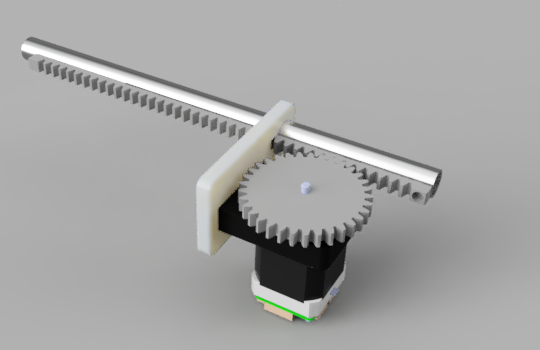
\includegraphics[height=7cm]{../photos/move_side_gear}
    \caption[moveside1]{Move side gear and gear rack}
    \label{fig:move_side_gear}
\end{figure}
% Todo: insert a picture of the meachaism that connects the tubes

\subsection{Turn Side}\label{subsec:turn-side}
The Turn Side is the part that rotates the player.
The turning motor is connected to a tube containing the smaller tube on which the player sits.
The larger tube contains a slit along its length, and the smaller tube has a pin that fits (a screw in this case) into the slit.
A render of the turning mechanism can be seen here:
\begin{figure}[H]
    \centering
    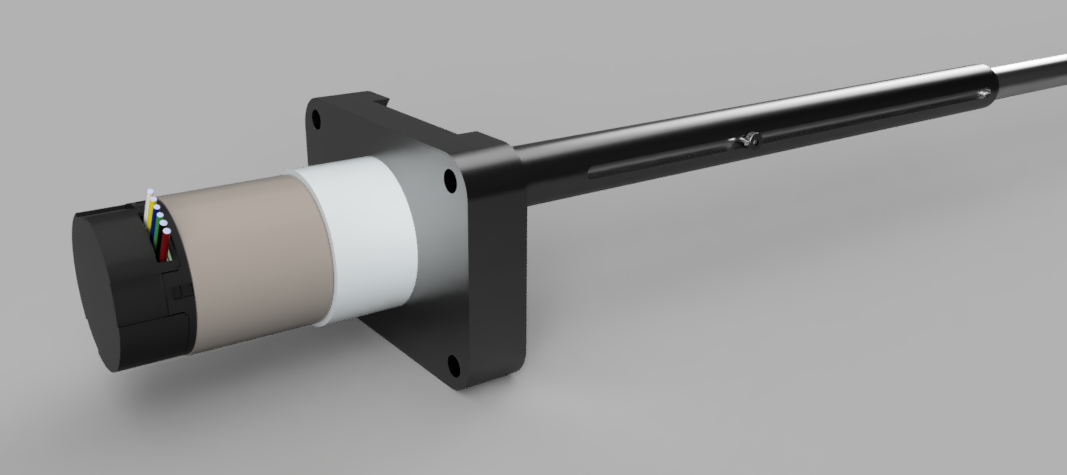
\includegraphics[height=7cm]{../photos/turn_side2}
    \caption[turnside]{Turn side with motor and slit}
    \label{fig:turn_side2}
\end{figure}